\section{FitzHugh-Nagumoモデル}
\subsection{FitzHugh-Nagumoモデルの定義}


\begin{align} 
\frac{dv}{dt} &= c\left(v-\frac{v^3}{3}-u+I_e\right)\\ 
\frac{du}{dt} &= v-bu+a 
\end{align}
ここで$a,b,c$は定数であり,$a=0.7, b=0.8, c=10$がよく使われる.$v$は膜電位で,$u$は回復変数(recovery variable)である. $I_e$は外部刺激電流に対応する.
まず必要なパッケージを読み込む.
\lstinputlisting[language=julia]{./text/neuron-model/fhn/003.jl}
変更しない定数を保持する \jl{struct} の \jl{FHNParameter} と, 変数を保持する \jl{mutable struct} の \jl{FHN} を作成する.
\lstinputlisting[language=julia]{./text/neuron-model/fhn/005.jl}
次に変数を更新する関数\jl{update!}を書く.ソルバーとしては陽的Euler法または4次のRunge-Kutta法を用いる.以下ではEuler法を用いている.Juliaではforループを用いて1つのニューロンごとにパラメータを更新する方がベクトルを用いるよりも高速である.
\lstinputlisting[language=julia]{./text/neuron-model/fhn/007.jl}
\subsection{FitzHugh-Nagumoモデルのシミュレーションの実行}
いくつかの定数を設定してシミュレーションを実行する.
\lstinputlisting[language=julia]{./text/neuron-model/fhn/009.jl}
結果を描画する.
\lstinputlisting[language=julia]{./text/neuron-model/fhn/011.jl}
\begin{figure}[ht]
	\centering
	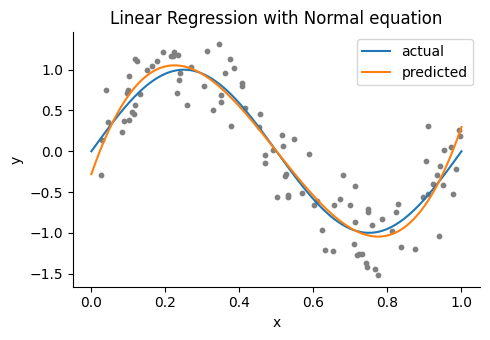
\includegraphics[scale=0.8, max width=\linewidth]{./fig/introduction/linear-regression/cell011.png}
	\caption{cell011.png}
	\label{cell011.png}
\end{figure}
発火回数を求める.
\lstinputlisting[language=julia]{./text/neuron-model/fhn/013.jl}
\subsection{相図の描画}
phase plot
\lstinputlisting[language=julia]{./text/neuron-model/fhn/015.jl}
\lstinputlisting[language=julia]{./text/neuron-model/fhn/016.jl}
\begin{figure}[ht]
	\centering
	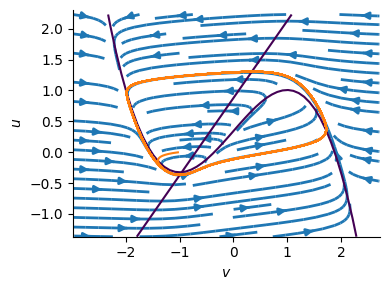
\includegraphics[scale=0.8, max width=\linewidth]{./fig/neuron-model/fhn/cell016.png}
	\caption{cell016.png}
	\label{cell016.png}
\end{figure}
